\chapter{Especificações e Arquitetura do Sistema}
\label{chap:arquitetura}
Durante todo o desenvolvimento do sistema, buscou-se não se utilizar dos modelos de arquitetura comumente empregados neste tipo de aplicação, que trabalham com grandes volumes de dados, um dos motivos vem a ser pela grande complexidade encontrada ao se trabalhar com módulos Apache como o Hadoop Common, Hadoop Distributed File System (HDFS), Hadoop YARN e Hadoop MapReduce, os quais dependendo de suas aplicações acabam por gerar dependências de outras ferramentas como Cassandra, Spark, ZooKeeper, entre outras que se mostram apesar de robustas, muito complexas e com uma curva de aprendizagem alta demais para serem usadas de imediato.

Outro motivo de grande valor para o desenvolvimento de uma nova arquitetura tem sido a empregabilidade de novas ferramentas utilizadas no lado \textit{backend}, por assim dizer, relacionado a organização dentro dos servidores, conceitos de desenvolvimento e bancos de dados que tem ganhado força dentro do mercado e se mostradas bem aplicáveis em projetos com grandes volumes de dados e alta disponibilidade, além de possuir uma baixa curva de aprendizagem, se comparadas com as tecnologias tradicionais.

\section{Micro Serviços}
\label{sec:microserviços}
Os Micros Serviços tem se tornado um padrão de projeto muito utilizado em aplicações de multiplataforma, pois através deste padrão este tipo de aplicação tem se tornado mais fácil de se desenvolver, demandando menos tempo. A ideia do padrão de Micro Serviços é desenvolver pequenos serviços autônomos que trabalham juntos, ou seja, um serviço possui uma única responsabilidade bem definida, mas para o funcionamento da aplicação por completa é necessário o uso de todos os serviços disponíveis dentro do domínio da aplicação. Sendo assim, um serviço pode ser um \textit{endpoint} de uma \textit{Application Programming Interface} (API), que pode retornar informações como todos os dados de uma tabela.~\cite{newman2015building}

\section{CQRS}
O \textit{Command Query Responsibility Segregation} (CQRS) é um padrão de desenvolvimento que descreve como separar as operações de leitura e escrita em diferentes modelos, sendo que para a leitura é utilizada a \textit{Query model} e para outros comandos como atualização e inserção de dados é utilizado o \textit{Command Model}, os quais compartilham da mesma base de dados, como mostra a figura \ref{fig:cqrs}.

\begin{figure}[!h]
\caption{\label{fig:cqrs} Arquitetura CQRS}
\begin{center}
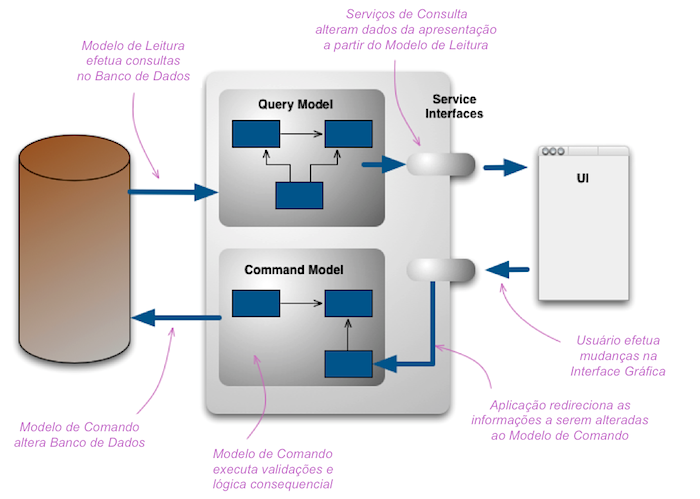
\includegraphics[scale=0.5]{cqrs}
\end{center}
\legend{Fonte: \citeauthor{cqrs}, \citeyear{cqrs}} 
\end{figure}

Este padrão foi desenvolvido tendo em vista que ao se criar novas regras de leitura e escrita, novas formas de representação das informações são criadas, o que já não faz mais sentido manter em um único modelo quando se fala em responsabilidade única, este é um padrão que adiciona grande complexidade ao projeto, portanto só deve ser utilizado caso as regras empregadas na leitura e escrita passem a ser complexas, não havendo um padrão fixo para todos os casos, é necessário adaptá-la ao problema que se deseja resolver.~\cite{cqrs}

\section{Docker Engine}
\label{sec:docker}
O Docker é uma plataforma aberta criada com o intuito de tornar mais ágil o desenvolvimento, implantação e execução de aplicações em ambientes isolados, além de ser multiplataforma, tudo isso através do conceito de conteinerização e imagens, em que numa imagem se tem todos os arquivos necessários para a criação de um contêiner, este por sua vez, possui a aplicação encapsulada  e funcionando.

Desta forma se tem uma grande flexibilidade para trabalhar com as aplicações, pois estas irão funcionar tanto em um notebook, quanto em um mainframe. Este conceito de contêiner se assimila ao processo de criação de máquinas virtuais, onde se tem todo o sistema operacional virtualizado, já o Docker realiza uma virtualização á nível do sistema operacional, mantendo um único kernel no \textit{host} executando processos (contêineres) de forma isolada, isso é possível através do uso de \textit{namespaces}, fazendo com que um processo só tenha acesso a recursos de outro se isso for explicitamente configurado na criação dos ambientes. Para que não ocorra a exaustão de recursos no \textit{host}, o Docker se utiliza de \textit{cgroups} do kernel, responsável por criar limites de hardware para os processos, evitando o uso exagerado de recursos por apenas um processo. A figura \ref{fig:arqdocker} apresenta a organização a nível de sistema operacional de um \textit{host} utilizando Docker.~\cite{docker}

\begin{figure}[!h]
\caption{\label{fig:arqdocker} Arquitetura Docker}
\begin{center}
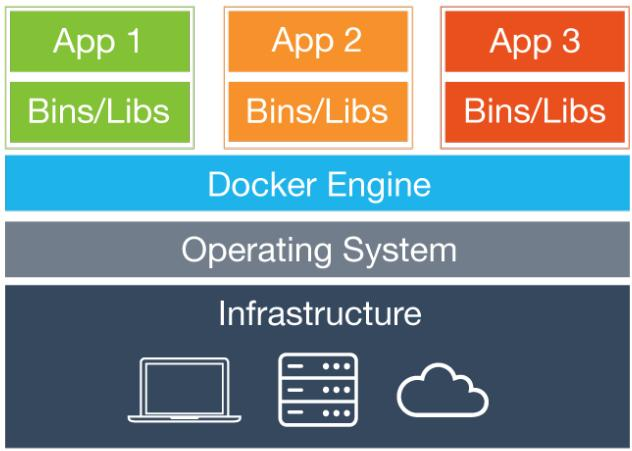
\includegraphics[scale=0.3]{arqdocker}
\end{center}
\legend{Fonte: \citeauthor{docker}, \citeyear{docker}} 
\end{figure}

O Docker tem ganhado fama no mercado, principalmente pelos profissionais de infraestrutura, pois ele tem facilitado o trabalho destas pessoas, fazendo com que elas economizem tempo para realizar a instalação de um software, não necessitando mais se preocupar com todas as dependências e ferramentas necessárias para o funcionamento do software, basta apenas se utilizar uma imagem da aplicação e transformá-la em um contêiner em qualquer ambiente que se esteja. Comumente o Docker não é utilizado isoladamente, pois o que traz a ele grande facilidade ao se trabalhar com contêineres é a junção de todas as suas ferramentas, as quais serão descritas a seguir.~\cite{docker}

\subsection{Docker Compose}
Com o aumento da complexidade do ambiente em que se está hospedada a aplicação, surgem as necessidades de se criar mais contêineres, tornando o seu gerenciamento um tanto quanto complicado, é neste cenário que se aplica o Docker Compose, uma ferramenta que trabalha juntamente com o Docker, ele se caracteriza por definir e executar múltiplos contêineres, pois através do uso de um arquivo que descreve todos os contêineres e configurações necessárias para o funcionamento de uma aplicação por completa, o Docker Compose tem a capacidade de criá-los, reiniciá-los e desligá-los quando necessário, facilitando assim o uso de contêineres.~\cite{docker}

\subsection{Docker Swarm}
Como visto até aqui, Docker Engine é o responsável pela arquitetura de criar e manter em funcionamento os contêineres, além de armazenar as imagens, o Docker Compose leva a responsabilidade da criação e remoção de múltiplos contêineres, facilitando o gerenciamento destes, por fim se tem o Docker Swarm a qual tem a função de gerenciar o \textit{cluster} de contêineres, ele pode ser considerado como um orquestrador de contêineres como mostra a figura \ref{fig:dockerswarm}, especificando quais máquinas e contêineres farão parte deste \textit{cluster}, sendo que muitos destes contêineres podem terem sidos criados a partir de um Docker Compose.   

\begin{figure}[!h]
\caption{\label{fig:dockerswarm} Docker Swarm}
\begin{center}
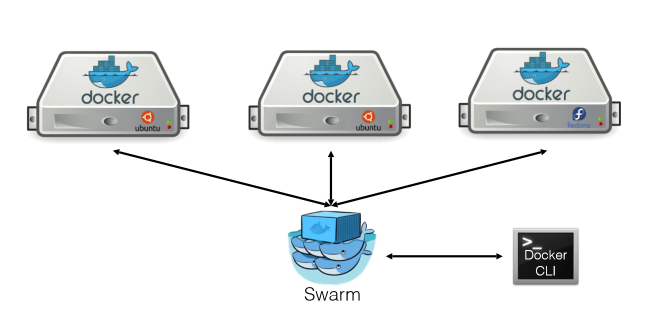
\includegraphics[scale=0.5]{dockerswarm}
\end{center}
\legend{Fonte: \citeauthor{dockerswarm}, \citeyear{dockerswarm}} 
\end{figure}


É o Docker Swarm que aplica todo o conceito de escalabilidade à aplicação conteinerizada, pois ela tem a capacidade de criar novas réplicas de contêineres de acordo com a necessidade, ou até os limites pré estabelecidos, é ele também que aplica o conceito de distribuição de cargas entre os contêineres que estão em funcionamento, podendo estes estarem na mesma máquina ou não, no caso de estarem em outra máquina o gerenciamento do Docker Swarm só é possível através da troca de \textit{tokens} entre elas formando um \textit{cluster} com contêineres homogêneos ou heterogêneos. É desta forma que é criado todo o ecossistema da arquitetura Docker, como pode ser visto na figura \ref{fig:ecossistemadocker}.~\cite{dockerswarm}  

\begin{figure}[!h]
\caption{\label{fig:ecossistemadocker} Ecossistema Docker}
\begin{center}
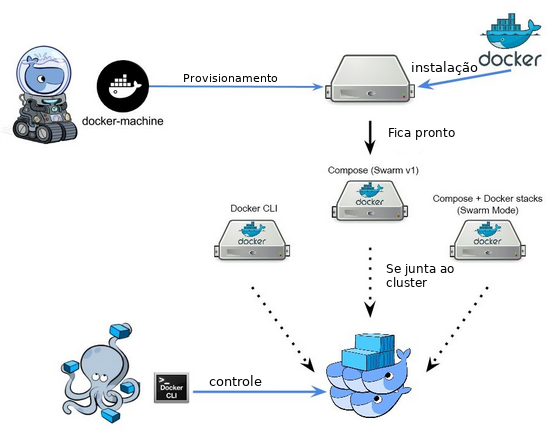
\includegraphics[scale=0.5]{ecossistemadocker}
\end{center}
\legend{Fonte: \citeauthor{dockerswarm}, \citeyear{dockerswarm}} 
\end{figure}

\section{Redis}
\label{sec:redis}
Redis é um banco de dados No-SQL destinado ao armazenamento em memória de dados no tipo chave-valor, utilizado para manter cache das aplicações, nesse cache podem ser armazenados \textit{hashs}, \textit{strings}, \textit{bitmaps}, listas e \textit{Hyperloglogs}, estes dados tem uma data de expiração após serem persistidos no Redis, por ser um banco de dados em memória, as ações de escrita e leitura se tornam mais rápidas do que uma leitura ou escrita em disco, dando maior \textit{performance} ás aplicações nas quais ele é implantado.~\cite{da2015redis}

\section{Clojure}
Apresentada ao público em 2007 ela foi desenvolvida visando a construção de aplicações multitarefa, aproveitando os recursos da máquina virtual Java (JVM), mas diferente do Java em que se escreve códigos orientado a objetos, em Clojure se tem códigos escritos em linguagem funcional, em que cada função é especializada em sua tarefa, sendo que a resolução de problemas se dá pela integração destas funções.

Algo que faz Clojure uma linguagem diferente das outras é que valores são imutáveis, isso resolve o problema que se tem de compartilhamento de memória quando usada várias \textit{threads}, outra funcionalidade interessante é a criação de macros, que é o equivalente a criar novas funcionalidades dentro da linguagem, algo muito útil para adequar a linguagem ao problema a ser solucionado. Além de tudo assim como o Ruby possuí o gerenciador de pacotes rake e o Java o Maven, Clojure possui o Leiningen, que gerencia os pacotes necessários para o seu funcionamento, além de disponibilizar um \textit{prompt} de comando para teste de trechos de código, similar ao pip do Python.~\cite{hickey2010clojure}

\section{Kafka}
O Kafka se caracteriza por ser uma central de mensagens distribuídas, em que todas as informações passam por ele antes de alimentarem um banco de dados, Data Warehouse ou algum outro sistema de análise de dados, dentre as suas vantagens estão a sua rapidez, alta escalabilidade e redundância, permite uma grande quantidade de conexões persistentes dos usuários , além de apresentar uma grande resiliência tendo a capacidade de se recuperar após a ocorrência de falhas. Desta forma o Kafka se torna ideal para comunicação e integração de componentes em sistemas de larga escala.

Seu funcionamento se dá através de partições sobre tópicos diferentes (como se fossem mensagens relacionadas a cada assunto, ou ainda pode-se comparar as tabelas de um banco relacional) que podem estar em diferentes máquinas, estas partições armazenam uma fila de mensagens, tendo cada uma delas um número identificador imutável que segue a ordem da fila, um consumidor dessa fila de mensagens tem a possibilidade de ler qualquer mensagem que esteja na fila através o seu identificador, um consumidor também pode consumir mensagens de diversas partições como mostra na figura \ref{fig:kafkatopicos}. As mensagens que chegam ao Kafka ficam armazenadas por um período de tempo configurável, não possuindo algo que informe se a mensagem foi lida ou não, apenas mantém pelo período estabelecido, caso o período seja menor ao período em que será feita a leitura pelo consumidor, essa mensagem será perdida

\begin{figure}[!h]
\caption{\label{fig:kafkatopicos} Partições do Kafka}
\begin{center}
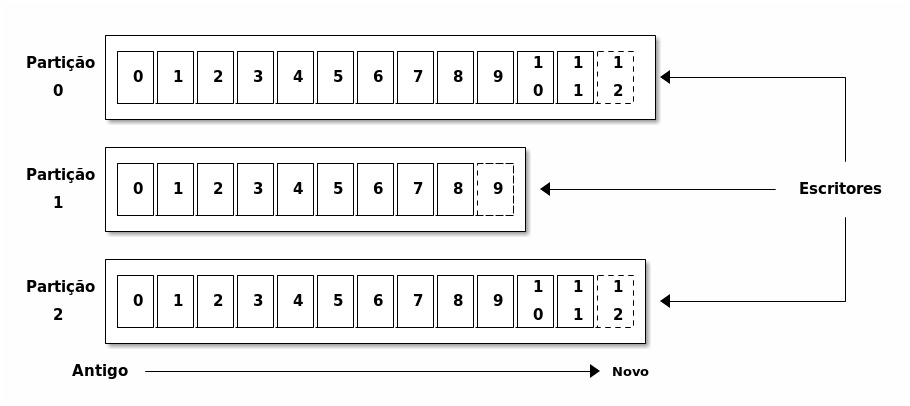
\includegraphics[scale=0.7]{kafkatopicos}
\end{center}
\legend{Fonte: \citeauthor{kafka}, \citeyear{kafka}} 
\end{figure}

Além da organização das mensagens dentro de partições, se tem ainda a organização de partições dentro de \textit{brokers}, onde se tem partições  chamadas de líderes e réplicas, no processo de produção de mensagens como apresentado na figura \ref{fig:kafkaproducao} o produtor escreve na partição líder, esta então gera cópia nas partições réplicas que podem estar em outros \textit{brokers} e em outras máquinas, desta forma se mantêm a consistência das mensagens e um alto nível de paralelismo, pois no processo de leitura o consumidor faz uma requisição para ler e a partição que está disponível retorna a mensagem para ele.~\cite{kafka}

\begin{figure}[!h]
\caption{\label{fig:kafkaproducao} Processo de escrita do Kafka}
\begin{center}
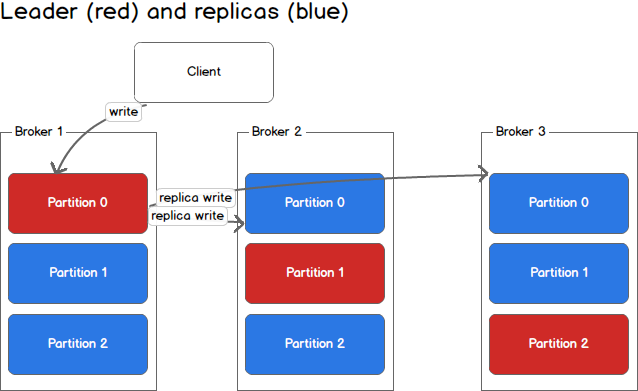
\includegraphics[scale=0.5]{kafkaproducao}
\end{center}
\legend{Fonte: \citeauthor{kafka}, \citeyear{kafka}} 
\end{figure}

\section{MongoDB}
MongoDB é um banco de dados orientado a documento, organizado em coleções de dados, aos quais se permitem operações de leitura e escrita, substituindo o conceito de linhas dos bancos relacionais por documentos, uma das grandes vantagens deste modelo é a fácil escalabilidade possível de se empregar, além da grande flexibilidade que se tem, pois não são pré-definidos identificadores, tamanhos ou tipos de dados para os documentos armazenados.

Dentre as funcionalidades dele se destacam a indexação através de texto o que mantêm uma boa \textit{performance} na execução de \textit{queries}, agregações complexas através de pedaços mais simples de código, tipos especiais de coleções suportando tamanhos fixos, suporta também o armazenamento de grandes documentos além de metadados. Seu funcionamento difere aos de bancos relacionais por não possibilitar as funções como \textit{joins}, ou seja, para utilizá-la é preciso que se armazene dados completos em um único objeto, pois quando se tenta utilizá-lo similar a um banco relacional toda a \textit{performance} da ferramenta quanto as buscas se perde.~\cite{chodorow2013mongodb}

\section{Datomic}
Assim como o MongoDB ele é um banco de dados não relacional, mas com um conceito diferente, adaptado para as novas demandas de serviços em nuvem com arquitetura \textit{Software as a Service} (SaaS), Datomic é um banco de dados orientado a fatos, com o grande diferencial de que dados nele persistidos se tornam imutáveis, isto não significa que não se pode alterar dados, mas o que acontece é um versionamento dos dados, desta forma é possível se ter um histórico do objeto persistido com todas as alterações já realizadas sendo a última versão o dado de maior veracidade.  

Possui como características separação dos conceitos de leitura e escrita, forte garantia transacional na escrita, noções de imutabilidade expressas por bases de dados estritamente incrementais, utiliza para as consultas de dados a linguagem Datalog, como é mostrado um exemplo da linguagem na figura \ref{fig:datalog} que é estruturada baseada em lógica permitindo consultas complexas incluindo \textit{joins} inferidos.~\cite{datomic} 

\begin{figure}[!h]
\caption{\label{fig:datalog} Exemplo da linguagem Datalog}
\begin{center}
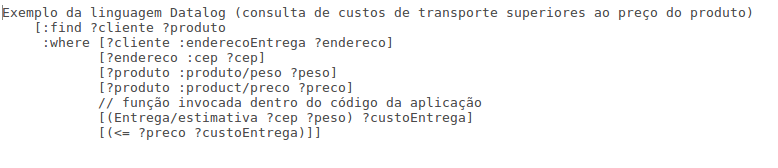
\includegraphics[scale=0.6]{datalog}
\end{center}
\legend{Fonte: \citeauthor{datomic}, \citeyear{datomic}} 
\end{figure}

\section{Arquitetura do Sistema}
Durante o desenvolvimento do projeto buscou-se utilizar do padrão de micro serviços, com cada um deles encapsulado dentro de um contêiner com responsabilidade única, sendo utilizado um arquivo Docker Compose, mostrado na figura \ref{fig:dockercompose} para sua criação e o Docker Swarm para realizar todo o gerenciamento de carga da aplicação, o \textit{cluster} de contêineres é apresentado na figura \ref{fig:dockerps}, a escolha de se utilizar micro serviços conteinerizados se deu pela grande facilidade com que se pode criar, remover e escalar toda a aplicação, por exemplo se em algum momento um serviço em específico está sendo mais utilizado que os demais, automaticamente podem ser criadas réplicas deste serviço para atender as demandas.~\cite{dockerswarm}

\begin{figure}[!h]
\caption{\label{fig:dockercompose} Arquivo Docker Compose}
\begin{center}
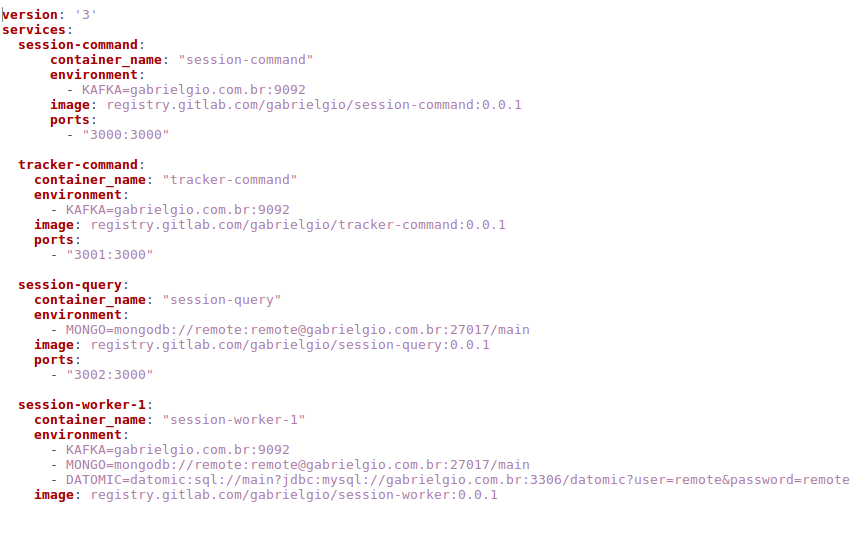
\includegraphics[scale=0.5]{dockercompose}
\end{center}
%\legend{Fonte: SOUZA} 
\end{figure}

\begin{figure}[!h]
\caption{\label{fig:dockerps} \textit{Cluster} de contêineres}
\begin{center}
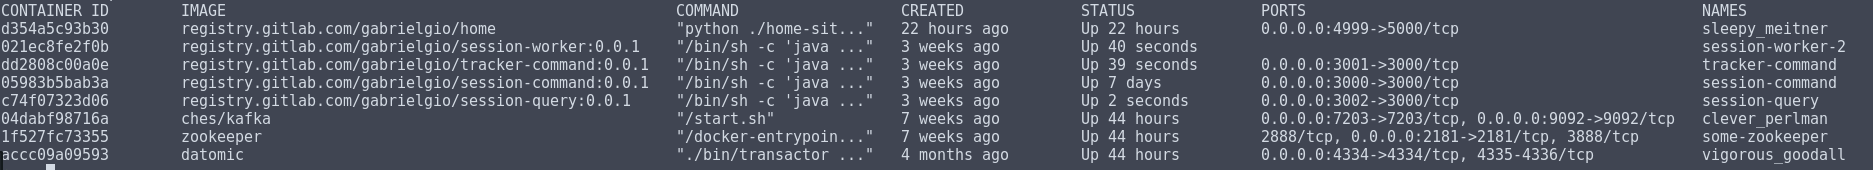
\includegraphics[scale=0.2]{dockerps}
\end{center}
%\legend{Fonte: SOUZA} 
\end{figure}

Utilizou-se também do padrão CQRS para a execução das operações de escrita e leitura, utilizado por se tratar de um sistema ao qual as regras tendem a aumentar sua complexidade, e assim estando no padrão CQRS a aplicação já estará pronta para suportar estas demandas. Para conhecimento da arquitetura por completa será analisado o fluxo de dados seguido pelo dado objeto a seguir, o qual é criado assim que um carro é ligado e faz uma requisição para se conectar a infraestrutura (iniciar uma nova sessão) no serviço de \textit{Command}:
\begin{lstlisting}
{
	"hd-id": "abcd1234",
	"model": "zyz",
	"brand": "123"
}
\end{lstlisting}

\subsection{\textit{Command}}
Operações de leitura, escrita e remoção passam por este serviço, escrito em Clojure devido ao seu alto paralelismo, que validará com as regras de negócio as informações recebidas e se passarem por esta fase, as informações serão inseridas em forma de texto, na fila de mensagens do Kafka para serem inseridos no banco de dados juntamente com um identificador da sessão criada para este carro, o dado enviado ao Kafka é apresentado a baixo:
\begin{lstlisting}
{
	"command": "create_session",
	"session-id": "{uuid}",
	"hd-id": "abcd1234",
	"model": "zyz",
	"brand": "123"
}
\end{lstlisting}

\subsection{\textit{Worker}}
Após a inserção da mensagem na fila do Kafka um outro serviço chamado de \textit{Worker} que monitora se existem mensagens a serem lidas no Kafka, irá ler esta mensagem e salvá-la banco de dados, neste caso por ser uma informação apenas de sessão será salvo apenas no MongoDB, mas para o caso de um novo cadastro de veículo ou alteração do mesmo, este serviço salvaria primeiramente no Datomic, o qual armazena dados históricos e posteriormente no MongoDB, o qual terá a informação imediata sobre o veículo, juntamente com esta informação de sessão o serviço de \textit{tracking} estará atualizando dados referentes a localização do veículo, como pode ser visto no objeto persistido no MongoDB apresentado a seguir: 
\begin{lstlisting}
{
	"session-id": "{uuid}",
	"hd-id": "abcd1234",
	"model": "zyz",
	"brand": "123",
	"location": {"x": 46.121, "y": 12.0213},
	"gas-lvl": 74
}
\end{lstlisting}

Esta estratégia de se salvar em dois bancos de dados faz com que Datomic fique armazenados todas as informações relevantes para se manter um histórico do veículo, mantendo a veracidade de dados sobre a entidade, já no MongoDB se tem os dados em tempo real e como pôde ser visto a grande vantagem do banco não relacional está na rapidez com que esse dado poderá ser buscado, pois em um banco relacional provavelmente se teria uma tabela para localizações e uma para dados do veículo, necessitando de funções de agregação de dados para se ter o objeto completo, desta forma, no banco não relacional todas as informações já estão agrupadas, se ganhando muito em velocidade.

\subsection{\textit{Tracking}}
O serviço de \textit{tracking} é o responsável por receber informações do veículo, como posição e velocidade, dentre algumas informações sobre o estado do carro, e colocá-las na fila de mensagens do Kafka, para serem inseridos pelo serviço \textit{worker} no MongoDB, juntamente com as informações de sessão do carro. 

\subsection{\textit{Query}}
Finalizado o processo de inserção de dados, o processo de leitura se dá pelo serviço de \textit{query}, o qual recebe a requisição do usuário e busca dados diretamente no MongoDB retornando assim as informações requisitadas, consultas realizadas no Datomic estão relacionadas com as análise de dados do Big Data, pois é lá que se formará a grande massa de dados possíveis de serem analisadas com o decorrer do tempo.

\subsection{Interface do Usuário}
Esta vem a ser o dispositivo implantado no carro que tem a função de se ligar aos sensores do carro, a fim de mandá-las para a infraestrutura, juntamente com a localização instantânea do veículo. Esta interface não é contemplada pelo projeto, mas é essencial para o seu funcionamento prático.

\subsection{Visão Geral}
De forma geral se tem um fluxo de dados para inserção como visto na figura \ref{fig:insert} e o fluxo de dados para leituras apresentadas na figura \ref{fig:select}, a estrutura geral de toda arquitetura é representada na figura \ref{fig:estruturageral}.

\begin{figure}[!h]
\caption{\label{fig:insert} Fluxo de dados para inserção}
\begin{center}
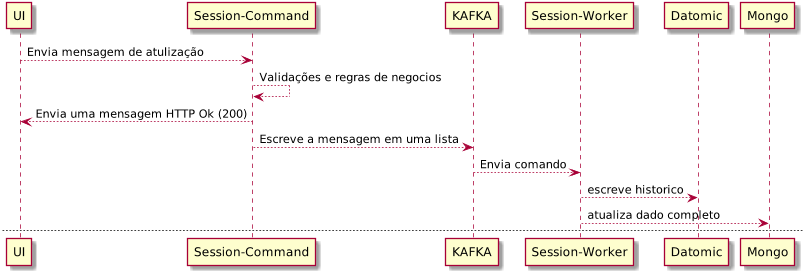
\includegraphics[scale=0.5]{insert}
\end{center}
%\legend{Fonte: SOUZA} 
\end{figure}

\begin{figure}[!h]
\caption{\label{fig:select} Fluxo de dados para leitura}
\begin{center}
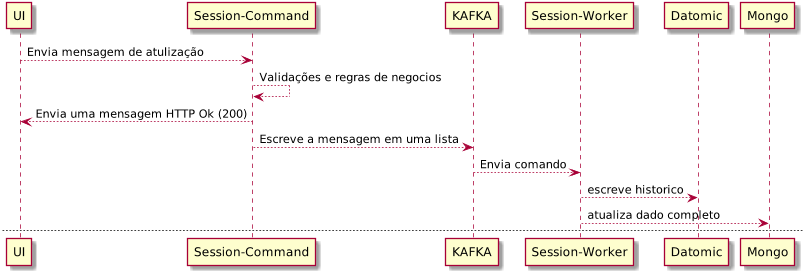
\includegraphics[scale=0.5]{select}
\end{center}
%\legend{Fonte: COELHO} 
\end{figure}

\begin{figure}[!h]
\caption{\label{fig:estruturageral} Estrutura Geral da Arquitetura}
\begin{center}
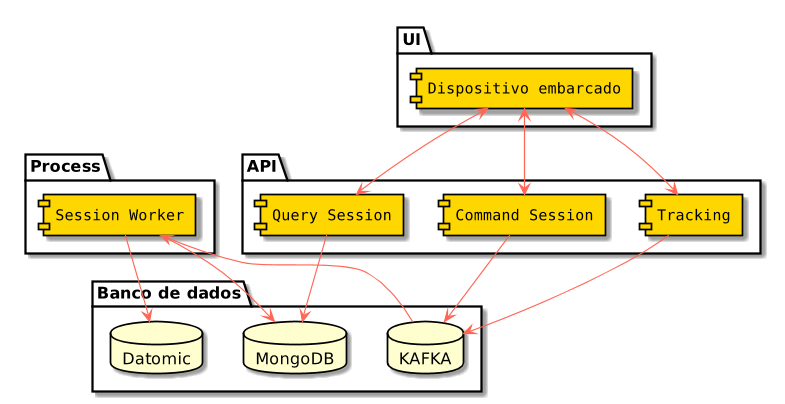
\includegraphics[scale=0.5]{estruturageral}
\end{center}
%\legend{Fonte: COELHO} 
\end{figure}
